\documentclass[12pt]{article}
\usepackage{setspace,graphicx,amsmath,geometry,fontspec,titlesec,soul,bm,subfigure}
\titleformat{\section}[block]{\LARGE\bfseries}{\arabic{section}}{1em}{}[]
\titleformat{\subsection}[block]{\Large\bfseries\mdseries}{\arabic{section}.\arabic{subsection}}{1em}{}[]
\titleformat{\subsubsection}[block]{\normalsize\bfseries}{\arabic{subsection}-\alph{subsubsection}}{1em}{}[]
\titleformat{\paragraph}[block]{\small\bfseries}{[\arabic{paragraph}]}{1em}{}[]
\setmainfont{Times New Roman}
\renewcommand{\baselinestretch}{1.15}
\renewcommand\contentsname{Inhaltverzeichnis}
\geometry{a4paper,left=2.5cm,right=2.5cm,top=2.5cm,bottom=2.5cm}
\begin{document}
	\newpagestyle{main}{            
		\sethead{}{Kapitel 4}{} 
		\setfoot{}{\thepage}{}
		\headrule
		\footrule
			}
	\pagestyle{main}
\tableofcontents
\newpage
\section{Absteckung und Abnahme im Hochbau}	
\subsection{Einleitung, Definitionen und Anforderungen}
Hochbau: Teilgebiet im Bauwesen, das sich der Planung und der Errichtung von Bauwerken befasst, die mehrheitlich oberhalb der Geländelinie liegen, z.B. Wohnhäusen, Industrianlagen, Brücken, Türme. \newline
\newline
Definition Bauwerkachsen: sind Raumachsen(häufig getrennt nach Lage und Höhe), die für die Herstellung einer Baumaßnahme in ein Baunetz anzurechnen und in der Örtlichkeit abzustecken und umzusetzen sind. Beispiel: Brückenachsen, Baulinien, Geländeachsen oder Begrenzungslinien.\newline 
\newline
Abstecken: Übertragung von projektierte geometrische Großen in die Ortlichkeit. Im Bauwesen meist Achsen oder Größen, die sich auf Achsen/Bauwerkachsen beziehen.\newline
\newline
Anforderung: hinsichtlich Lage und Form unterscheiden!\newline
\newline
Äußere Geometrie: Lage und Form des Bauwerks bzw. Bezug zu übergeordnete Festpunkte.
\begin{itemize}
\item geringe Anforderung
\item Genauigkeitmaße enthalten auch Anteile aus Genauigkeit der Festpunkte.  
\end{itemize}
Innere Geometrie: Lage der Punkte eines Bauwerks zueinander oder mehrere Bauwerke zueinander. z.B. Gradlinigkeit von Achse.
\begin{itemize}
\item höhere Anforderunge
\item Genauigkeitsmaße enthalten nur geometrische Informationen(aus Konfiguration) ohne Unsicherheit des Datums.
\end{itemize}
Wichtig: Parallelität der Schienen, Gradlinigkeit der Schienen(Innere Geometrie)\newline
Unwichtig: Lage der Schienen relativ zu Bauwerk(Äußere Geometrie)\newline
\newline
Unterteilung in:
\begin{itemize}
\item Lageabsteckung + Geschißabsteckung 
\item Höhenabsteckung
\end{itemize}
(gilt für Sondernetze und für Absteckung)
\subsection{Ingenieurgeodäsie Sondernetze}
Baulagenetze:
\begin{itemize}
\item Polygonzüge: beideseitig eingeschlossen oder Ringpolygon. Absteckung von Polygongpunkt aus oder durch frei Stantionierung.
\item Dreiecknetz / Poläres Netz: gesteigerte Genauigkeit und vor allem Zuverlässigkeit. Absteckung direkt vom Netzpunkt, oder von einem Verdichtungspunkt oder durch freie Stationierung.
\item Orthogonal Netze
\end{itemize}
Genauigkeit von Baulagenetzen:
\begin{itemize}
\item stark abhängig von Anforderungen des Auftraggebers.
\item Etwa von den Funktion 10 genauer als die Absteckung
\item Anforderungen sind immer relativ, also an die Entfernung geknüpft. 
\item Wenn nicht bekannt, dann Angaben aus der Literatur.
\end{itemize}
Höhennetze:
\begin{itemize}
\item nivelliertische Bestimmung
\item möglichst stabile Punkte in Objekenähe
\item Anschluss aus übergeordnete Netz
\end{itemize}
Einrechnung eines Sondernetzes:\newline
A) Sondernetz, ohne Spannungen, Geometrie ungestört, lokal. \newline
B) Landesnetz / übergeordnete Netz: mit Spannung, global. \newline
$\longrightarrow$ Datumsfestlegung: (Alternativen) (zwangsfrei) freies Netz, weiches Datum.
\subsection{Lageabsteckung}
Absteckungsarten: \newline
A) Grobabsteckung
\begin{itemize}
\item in der Regel für Baugraben, Aushub.
\item Punkte werden durch Holzpflöcke vermarkt.
\item $\sigma_{x,y} < 2 \cdot 10^{-3} \cdot s + 5$ cm, z.B: bei $s=20$m, $\sigma<6,5$cm
\end{itemize}
B) Feinabsteckung \newline
Absteckung von Objektpunkte für Achsen, Gradienten, Flächen und Gebäudeecken sowie sonstige Geometrie. Beispiel: Schnurgerüst.
\begin{itemize}
\item Absteckung der Hauptachsen, die die Geometrie der Fundaments beschreiben. 
\item Holzkonstanktion wird durch Baubetrieb außerhalb der Baugrabe erfüllt.
\item Achsen wirden durch Nägel mit den Konstruktionen durch dem Vermessen hergestellt.
\item Ablotung erfolgt mechanisch an Kreuzungspunkte
\item wichtig sind Sicherungspunkte in Verlängerung der Achsen am besten im Sondernnetze intergiert. 2 Sicherungspunkte pro Achse zur der Nägel
\end{itemize}
Absteckverfahren: \newline
A) Polarverfahren
\begin{itemize}
\item Freie Stationierung oder polares Anhängen.
\item Soll-Richtungswinkel und Soll- Strecke können berechnet werden, da abzustreckende Koordinaten vorliegen.
\item $\sigma_P = \sqrt{\sigma_s^2 + s^2 \frac{2\sigma^2}{\rho}}$
\item Messung mit Tachymeter
\end{itemize}
B) Orthogonalverfahren
\begin{itemize}
\item mit Messband und Prisma / Kreuzscheibe
\item Genauigkeit ist gering
\end{itemize}
\begin{figure*}[ht]\centering
	\subfigure[Orthogonalverfahren]{
		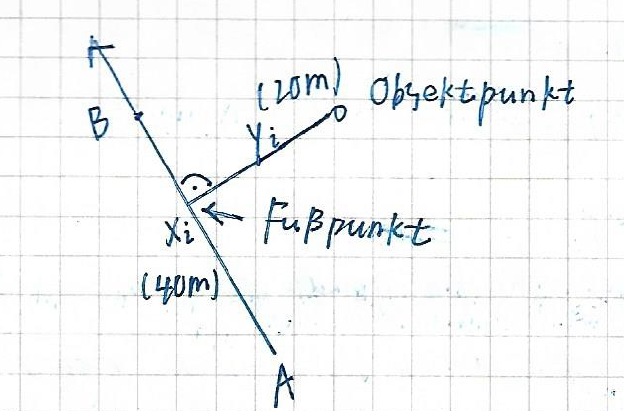
\includegraphics[width=0.65\textwidth]{Orthogonalverfahren.png}}
\end{figure*}
\begin{itemize}
\item $\sigma_{y,R}$ = Standardabweichung für den rechten Winkel
\item $\sigma_{x,s}\; \sigma_{y,s}$ = Standardabweichung der Streckenmessung
\item $\sigma_{x,F}$ = Standardabweichung des eingefulchteten Fußpunktes
\end{itemize}
\begin{equation*}
\sigma_p = \sqrt{\sigma^2_{x,s} + \sigma^2_{y,s} + \sigma^2_{y,R} + \sigma^2_{x,F}}
\end{equation*}
numerisch:
\begin{gather*}
\sigma_s = 5 \cdot 10^{-4} \; s \quad (Messband)\\
\sigma_{y,s} = 1\; cm \\
\sigma_{x,s} = 2\; cm \\
\sigma_{x,F} = 2\; cm \\
\sigma_w = 40 \; mgon \\
\sigma_{y,R} = \frac{40\; mgon}{\rho} \cdot 20m = 1,3\;cm \\
\sigma_P = 3,3\; cm
\end{gather*}
C) Bogenschnitt -/ Linsenschnittverfahren
\begin{itemize}
\item Nutzung zweier Messbänden durch Baubetrieb
\item einfaches Verfahren
\item geringe Genauigkeit
\end{itemize}
D) Winkelschnittverfahren (genaustes Verfahren)
\begin{itemize}
\item reines Winkelmessverfahren für Genauigkeiten in sub -mm Bereich
\item sehr zeitaufwendig
\item Theodolit zu Messung ausreichend
\end{itemize}
Vorgehensweise
\begin{itemize}
\item Absteckelemente sind Winkel $\alpha$ und $\beta$
\item Winkel $\alpha$ einstellen
\item einen Punkt A1 vor und einen Punkt A2 hinter dem abzusteckenden Punkt abstecken
\item beide Punkte durch Linie verbinden 
\item die P zed von $\beta$ mit $\beta$ und den Punkten B1 und B2 wiederholen
\item Schnittpunkt der Linie ist zum absteckenden Punkt
\end{itemize}
Genauigkeit: (siehe Vorwärtsschnitt)
\begin{gather*}
\sigma_P = \frac{1}{\sin \gamma} \sqrt{s_{AP}^2 + s_{BP}^2} \cdot \sigma_w \\
\end{gather*}
\begin{itemize}
\item $\gamma$: Schnittwinkel am Objectpunkt P, $\gamma = 200\; gong - (\alpha + \beta)$
\item $\sigma_{\gamma} = 0,3\; mgon \longrightarrow \sigma_w = \sqrt{2} \cdot \sigma_{\gamma}$
\item $\gamma = 120\; gon$(optimal) $\longrightarrow \sigma_P = 0,2\; mm$
\end{itemize}
E) Alignementsmethode
\begin{itemize}
\item Variantion des Winkelverfahren
\item optisches Einflachten von Punkten im Sondernnetz, dann Winkelmessung für Achschnitt Punkte
\item Genauigkeit wie D
\end{itemize}
Geschossabsteckung 
\begin{itemize}
\item Übertragung der Gebäudeachsen auf mehre Geschosse 
\item Feinabsteckung
\end{itemize}
A. Außerlotung
\begin{itemize}
\item Hochloten durch Theodolit, der in gut horizonten Zustand, die einzelne Achsen überträgt.
\item Herstellung des "Schnurgerüstes" für jedes Geschoss
\item einfache Instrumente, daher häufig von Betrieb durchgeführt.
\item Nachteil: große Platzbedarf
\end{itemize}
B. Innenlotung 
\begin{itemize}
\item Hochloten mittels Zenit- oder Nadirloten
\item Zenitlot realisiert Lotlinie zum Zenit(nach oben)
\item Nadirlot realisiert Lotlinie entgegengesetz zum Zenit(nach unter)
\item Absteckung der Punkten mit dem Tachymeter polar
\item Hohe Genauigkeit: $0,5mm / 100m \longrightarrow 5 \cdot 10^{-6} \Delta H \rightarrow$ \\ 
Anwendung für Hochhäuser, Kühltürme, hohe Türme
\end{itemize}
C. Freie Stationierung
\begin{itemize}
\item Freie Standpunktwahl in jeden Geschoß mit Anschluss Punkten im Baulagennetz
\item Hoher Platzbedarf von meist Ausführung durch Geodäten
\item Nachteil: Sichtbarkeit der Anschlusspunkte
\item heute Standardverfahren
\end{itemize}
Problem bei der Geschossabsteckung:
Einfluss des Stehachsfehlers: 1.Maximalfehler: Angabe der Libelle $20'' \approx 6mgon = v \longrightarrow$ Stehachsfehler $v=6mgon$ annehmen. \newline
\begin{equation*}
r_v = v \cdot \cot z \\
\end{equation*}
$v:$ Stehachsfehler, $r_V:$ Einfluss auf Zenitwinkel. \newline
Beispiel:\newline
1) Baugrabe
\begin{figure*}[ht]\centering
	\subfigure[Ander Grenze der Genauigkeitsanforderung bei der Feinabsteckung]{
		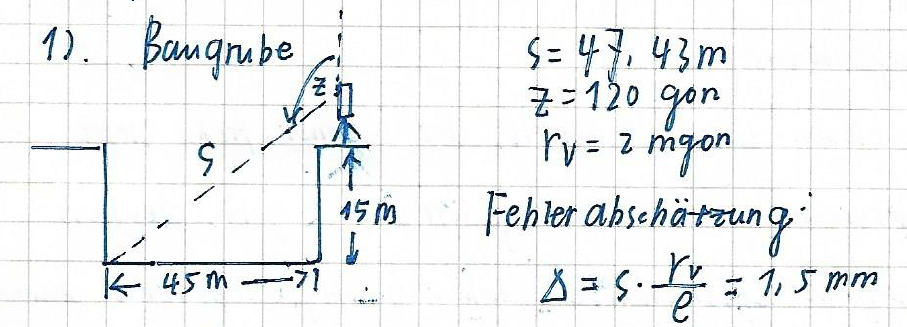
\includegraphics[width=0.65\textwidth]{Geschoss_1.png}}
\end{figure*}
\newline
\begin{figure*}[ht]\centering
	\subfigure[Außerhalb Feinabsteckungsgenauigkeitsgrenzen und bei hohen Genauigkeitsforderungen und froßen Höhen entscheidende Faktor]{
		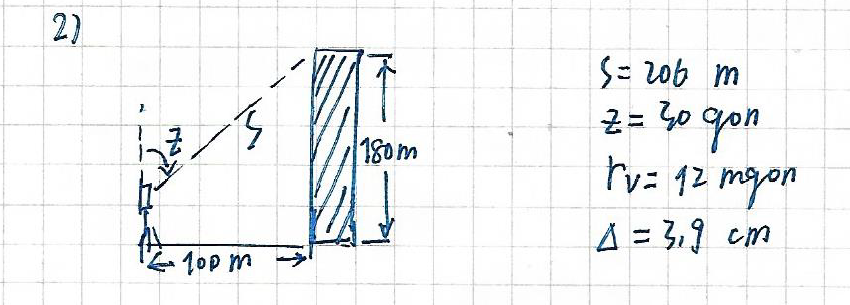
\includegraphics[width=0.65\textwidth]{geschoss_2.png}}
\end{figure*}
\subsection{Höhenabsteckung}
\begin{itemize}
\item ein oder mehrere Hohenbezugspunkte werden durch Nivellement bestimmt (z.B Höhenholze (HB) in Keller)
\item in der Geschossen: Kunststoffmarken oder Meterrisse(Marke in 1m Höhe) Landesnetzes
\item Messverfahren: Nivellement, Kalibrierte Strablmessbände und trigometrische Höhenübertragung
\item Genauigkeitsforderung: $HB \leq 2mm$, Marken/Meterrisse $\leq 4mm$ 
\end{itemize}
\end{document}
